In this chapter the team will evaluate different aspects of the projects. 
Everything from team collaboration, the project assignment, the cooperation with both customer and supervisor, to risks- and role assignments. There will also be discussed how the team tackled challenges during the project, and how the team handled the project management. Briefly explained the team will discuss why and how the outcome ended up being what it is today.
This chapter is split into three major parts, which is group evaluation, project evaluation and technology evaluation. 

%_______________________________________________________________________________
\section{Group evaluation}
In this section the team will elaborate on how the group functioned as a whole, and how the team collaborated. The team will also evaluate both the customer and the supervisor, before moving on to the evaluation of the goals the team sat at the beginning of this project. After this the team will evaluate the challenges met during this project and how this affected the work. At last the risk and role assignment will be evaluated.

\subsection{Team dynamics}
In this section is about how the group functioned as a whole, how the team communicated, the work distribution, and at last our motivation.

\paragraph{In general}
The group was randomly put together, and the number of people in this group was four.
Each person with different personalities and interests. A perfect atmosphere was not expected. Fortunately the team had no major conflicts, only constructive discussions. For the most part the team functioned well together, and offered each other help when needed. 
Overall the team feels like the team work, and progression of the project was good.

\paragraph{Communication}
Good communication within a team is important. For a team to perform it needs a safe and stable working environment. The importance of this was addressed early on. 
It was decided that every decision made in the group should be a result of a democratic process, which meant making decision by the majority vote. 

The communication was mostly done collocated. Mostly because of our agreement of sitting in the same work area as much as possible. This turned out to be a good rule most of the time. 
When every one was siting together it was never difficult to get help from the rest of the group. This enabled the tea, to quickly discuss points in doubt, and continuing with the work. This also gave the team a smoother work flow, a quicker progression, and it gave the team more time to revise and improve the work.

Because of completely different schedules, it was not always possible to sit collocated. Often there was a team member missing at working hours. There were a few situations where the team would have benefited from having the entire group present, but there was nothing the team could have done. Luckily it did not affect the project too much. The team solved the problem by using Facebook. If someone had other obligations, and they were not able to be present, then the team kept in contact through Facebook. This was a suitable solution since the team members were available online often. This made coordination an easier task, since all of the team members could respond as soon as possible. 

There were a few problems with the groups communication. The team were too much dependent on the team member responsible for the communication. The team did not always get copies of emails written to the supervisor or the customer. This caused a little confusions regarding the meeting hours from time to time. It was also the cause of important information coming a bit late. The team should have had more strict rules for this.

In hindsight the team is able to point out a couple of things that could have made the communication better. The team could have done more stand ups. The lack of stand ups was another problem caused by the different schedules. The team tried to solve this problem by having longer meetings when needed, or suggested by a team member. Still, the team should have had more clear rules about stand ups, and this could have made the communication easier. 
More communication with other groups taking this course was another idea that could have improved the team communication.
Although the tasks were different, the exchanging of ideas and sharing experiences on both group dynamics and processes could have affected the team in a positive way. 

The team also had some social gatherings to get to know each other better, and throughout the project the team got well known with each other. This made the communication easier for us as a team. By learning from each other, and learning to put aside differences, one can say that everyone has grown as individuals. In spite of a couple of bumps in the road, the team feel that the issue of communication was handled pretty well.

\paragraph{Work distribution}
The distribution of work was challenging at times. 
The team had little experience with image processing, and therefore it was hard to be sure about the exact work load. Naturally this also made it difficult to maintain a balanced workload throughout the project. 
In the beginning the team agreed on what needed to be done, and then group members had to take individual responsibility to perform work on the tasks they were comfortable with. 
Towards the ending of the project it was a bit stressful, because of troubles with the final demonstration video. Suddenly the team needed to spend more hours than expected. This is something the team should have anticipated, and the team should distributed the work a better.

\paragraph{Motivation}
All team members were very motivated. Everyone wanted to receive a good grade in this course, since the course was very relevant for us.In this course the team had to use knowledge from several different courses in previous years. Another motivation was the project assignment. The fact that the assignment was interesting increased our motivation and efforts. It was exciting and the team had the opportunity to learn something new. Our customer was also a great motivator, and by forcing us to deliver something at the end of each sprint, the team always felt like the milestones was reached. This way we always felt one step closer at the end of each sprint, and it became very motivating to continue the hard work. 

\subsection{Customer and project task} \label{txt:evaluation_customerandprojecttask}
Our customer, Peder Kongelf, was pleased with the results. During the last customer meeting he informed the team that the project goal was reached, which was to make the audience as a screen at a rock concert, and to do this using image processing.
This project was a proof-of-concept project, and if someone wanted to do further work on our application the only remaining parts would be performance and scalability. 
The team wanted to have a bigger "wow-effect" on the last video demonstration, but we did not have enough resources to conduct this. With the demonstration video it is only possible to see the potential the project has. All in all the customer was satisfied with this result and explicitly stated that team accomplished all required tasks. 

The team is very impressed with our customer. The project given to us for this course was extremely exciting. The team got to work with challenging and new technology, which was really great. The fact that the task was interesting increased our motivation and efforts. He had plenty of experience with working as an consultant, and he was eager to teach us as much as possible. The team also wanted to learn as much as possible from him. He gave us good advice through out the whole project. One of the best advices he gave was about working together as much as possible. Looking back the team realizes that otherwise communication challenges could have been much tougher. Our customer also helped us with the scrum methodology. He taught the team a lot about everything from epics, user stories, task, estimation, to reviews. All of this was extremely useful for the team.

Early on Peder suggested weakly meetings, which was good. He always gave the team great feedback, as well as giving an impression of having confidence in the team. Sometimes, because he had a great amount of work load him selves, the meetings where shortened. Still, he was involved and enthusiastic about the project. Of course the team expected some communication problems from time to time. This was challenges like confusion over meeting hours, but the team addressed these issues very smoothly. The final conclusion about the customer is that the team would not have been able to deliver this end result if not for the great effort and constant feedback from the customer. 

\subsection{Supervisor}
Almost every week the group met up with the supervisor. In these meetings the progress made by the group was presented, and the supervisors came with feedback on the report and other work. It was quite useful to know whether the team needed to increase the work speed or not. 
The supervisors also gave feedback on the content of our report, which was useful for the team.

Before the meetings the team sent out a meeting invitation to the supervisor.
If there were something in particular the team had questions about, then the relevant documentation was emailed to the supervisor before the meeting, so the he could get a chance to look at it before the meeting.

In the beginning the meetings were useful in order to assure that the team were on the right track. After a while there was less need for a weekly meeting, because the team had a better understanding of what the report should look like.
Maybe a shorter meeting would have been more sufficient for the middle part of the project 

The communication with the supervisor could have been better time to time. Especially there was a little misunderstanding when the supervisor had to travel to a conference, and some of the team members showed up to a canceled meeting. This was just little bumps in the road, and most of the time the supervisor was available, and gave us really valuable feedback, especially with the report. 

\subsection{Goals} 
In this section the team will evaluate the project goals, the group goals, and our personal goals, to see if the team achieved them. 

\subsubsection{Project goals}
\paragraph{Finish the project within the scheduled timetable}
The team finished the project within scheduled timetable. It was a little stressful towards the ending, but this goal was reached.
\paragraph{Finish the project with the specified requirements}
The project was finished with the specified requirements, and the team made a demonstration video for the final presentation to show off the system. This goal the team achieved. 

\subsubsection{Group goals}
\paragraph{Receive a good grade or a good recommendation}
At this stage it is difficult to determine whether this goal was achieved or not. Looking back at setting these goals the team realizes that setting more measurable goal would have been better. The team has learned from this, and will take this experience with us fore future projects.

\subsubsection{Personal goals}

\paragraph{Agnethe}
One of my personal goals was to learn more about group dynamics and collaboration. This I have definitely done. Working as a team can be challenging at times, and I have learned a lot from this experience. Another goal of mine was to learn more about writing reports. Writing this huge report has thought me a lot about technical writing, and I feel more prepared for writing reports in other courses later on. A goal that is hard to determine at this point is whether im better at holding presentations since this report is supposed to be finished before holding the final presentation. The last goal I would like to mention is that when I wrote the goals in the beginning of this course I wrote that  there is a great chance that I would work as an IT- consultant. Looking back at this and I realize that I really enjoyed this experience. Working as an IT-consultant is something I would like for the future. 

\paragraph{Jan}
When looking back on the whole project timespan now I see that one of the main purpose of this course was to teach students to cooperate and communicate both together in development team and also with the other project related authorities such as the supervisor and the customer. I gained the idea of what does it take to work under agile methodology Scrum and I appreciate this experience as I might come across it in my future carrier. I also improved my skills as far as the Java/Android programming is concerned but not as much as I expected mostly due to the fast tempo and the need of doing other tasks. Even thought sometimes boring I appreciate that writing technical documentation was a part of this project as I definitely improved my English writing skills. As for the course itself I must admit I was a bit disappointed by the organization and the lack of lectures and/or other sources of information related to the project. I enjoyed working with my team colleagues though and to conclude I feel this course was beneficial for me.

\paragraph{Milos}
After 13 weeks of team work my primary goals and expectations from this course have been fulfilled. I learned how to be part of the team and how to collaborate with other people in achieving common goals. Further more I was enjoying working with new teammates. Overall atmosphere was great, team spirit was on high level and we even spent time together beside this project. For this reason, we were able to finish all of the set requirements and manage occurred risks and minor conflicts without big effort. Writing documentation helped me with technical English, just as expected, and practicing SCRUM gave me a picture of how real companies manage their development cycle. For me this project was absolute success and I will be proud to add it to my CV.

\paragraph{Tomas}
During this course, I have enormously improved my written English. 
It was also useful to learn about technical writing in English language, since some of the rules are different than in Czech.
Working in group and collaboration was sometimes difficult, due to different views of team members, and there is often need of compromises.
I have increased my knowledge in topic of architecture and software design and I have learned a lot of new diagrams.
Unfortunately due to the work distribution, my Android platform development skills have not improved as I expected, because other more knowledgeable team members were responsible for these parts.

\subsection{Challenges}
The team will in this section reflect on the challenges experienced, why they occurred, and what we could have done differently.

\paragraph{Time and time estimation}

Throughout the project, time restrictions has been a challenge because most of the members in the group have had other projects during the semester. Agnethe had two different projects in addition to the customer driven project. Milos also had another project that was quite time consuming in the beginning. Jan and Tomas also had another projects besides the customer driven project, and Jan also wanted to take Norwegian classes. All of this made it hard to find suitable working hours, and time. 

The actual amount of logged work fell a little short of the expected amount of hours. Still, the team were able to successfully execute the tasks  planned. The team also feels like the shortage of hours did not have any significant detrimental effect to the project. 

Regarding the time estimation, the team thinks the estimates were within reasonable bounds, but still it could have been better estimations for some of the user stories. To improve these time estimation the team could have done a better job using the planning poker. While reviewing this the team realizes that realistic time estimation is valuable, and that this project has taught us a lot about this.

\paragraph{Language and Cultural Barriers}

Within the team there were three different nationalities. The were one Norwegian, one Serbian and two Czechs. Since there were different nationalities the communication had to be done in English. English was spoken internally in the group. The communication with both the supervisor and the customer
was also done in English. It was a challenge to have all communication in English. Solutions and technical issues is probably easier to discuss in a persons native language. This caused challenges during the decision makings. It was spend more hours then expected discussing some issues, because it was hard to express everything in English. It was also hard to get a clear understanding of the different arguments. Sometimes Jan and Tomas switched to Czech, to be able to help each other. Sometimes it was easy to lose focus during discussions when the language was switched, but most of the time it was very useful and it progressed the discussion.

Since everyone was used to study at different universities, with different cultures, and with different ways of doing things. The team sometimes had different methods for solving problems. If the team could not reach a decision, it was decided to ask the supervisor or customer to get additional information, and then try to make a new decision. Very often this helped to shed new light on the situation. If the team still could not make a decision the majority vote was used. For the most of the time language and cultural differences was not a problem. Everyone was excited to learn, and teach each other. 

\subsection{Role assignment}
As mentioned earlier the role assignment were adapted a bit, so they could fit the project better. Also the roles assigned to each group member was more of a guideline, rather than a binding responsibility. This was mainly because for some of the team members, this was their first scrum project. Some of the roles required more experience and knowledge then the group member had. The team solved this problem by working together, and helping each other. 

Looking back at the role assignment it is not possible to deny that there are things that could have been differently. Since everyone was working with mostly unfamiliar technologies in the beginning, it might have been a good idea to make each of the role's responsibility more clear, and enforcing them in the early stages of the project. Also, the team could have have spent more time researching the roles actually needed. Even though it was decided to embrace this as an equal development team, the roles might have been useful for us it these improvements had been done. 

These are the roles assigned, and this is how they were evaluated.

\paragraph{Project Leader}
The project leader was supposed to be responsible for the project progression, and delegate tasks to the other team members. This did not work very well, because the tasks was prioritized by the customer. If one task was done, the team member had picked the task with the highest priority to do next. All of the team members took responsibility for the progression of the project, and tried to make sure that it went according to plan. The description of this role also claimed that the Project Leader had final call in arguments. This was not the case, since it was decided from the beginning that this as an equal development team.

\paragraph{System Architect}
The system architect was responsible for checking and analyzing all the layers in the product, but this was also something not only one person took responsibility for. 

\paragraph{Scrum Master}
The Scrum Master role was assigned to one person originally. Nevertheless, all team members took responsibility for following up on this. It became natural to suggest to have stand ups during working hours, since it was not always easy too keep track of what the other team members were working on. Having the whole team responsible for scrum methodology worked for this project, because of the team members having different schedules. 

\paragraph{Communication Responsible}
This is the only role that was used throughout the whole project. The reason for this is because it was easier for the team to keep track, and it was also easier for both the customer and supervisor to have only one person to communicate with.    

\paragraph{QA Responsible}
The QA was responsible for the quality of all documents and the end product. Still, the whole team felt responsible for delivering a product with good quality. The QA was also supposed to help determining if stories and acceptance criteria was well defined. For this project it was difficult because it was hard to do with little experience. A QA is also responsible for organizing testing, and this includes that unit tests are well written, provide developers with high level test cases for the stories, and performing exploratory testing on early builds. For this project the testing part was not a priority. All of the above resulted in that this role was not used.

\paragraph{Documentation Responsible}
This is a role that all team members took responsibility for. It was smart having one person responsible for setting up a good structure in the beginning. After a while everyone participated where they could. 

\subsection{Risk evaluation}
In this section the risks from the risk Table \ref{tab:risks} in the planning section, will be evaluated. Among these risks the team only experienced a few of them.

\paragraph{Sickness/Absence}
Some of the team members where exchange students, and they wanted to travel and experience Norway during the semester. Naturally it lead to some absence at times. When this happened the team members worked extra hard for this not to affect the project. This was also the solution if members got sick, and for this project this was a good solution. 

\paragraph{Coding problems}
To some extent the team experienced some coding problems, but the team figured it out. At the end it was possible for us to reach the project goals. This is a risk that probably occurs in most projects. Because of reflecting over the risks the team was prepared that might happen.

\paragraph{Testing problems}
This risk did not occur, since the customer told us not to focus on the testing part.

\paragraph{Changing requirements} 
The team did not experience problems with requirements changing too much. The communication with the customer was really good, and possibly because of the reflection over this risk, the problem was avoided.

\paragraph{Dead end with technologies}
While doing research for existing solutions the team experienced difficulties. The team could not find a good existing solution. Luckily the team found OpenCV, and by using this it was possible to finish the project. 

\paragraph{Unrealistic time estimation}
It was not easy to estimate all of the user stories. Sometimes the team underestimated and other times the team overestimated. Towards the ending of the project it was a bit stressful, but mostly this did not affect this project.

\paragraph{Customer too ambitious}
The team did not experience that the customer was too ambitious. The reason for this was because the communication with the customer through out the project was very good. The team and the customer had good sprint reviews, and planned the next sprint together.

\paragraph{Hardware problems}
The team had some hardware problems. For this project the team were dependent on borrowing phones to be able to test the system. It was not easy to borrow phones from a lager amount of friends at the same time. The hardware problem was that the team did not have enough resources. Luckily the team was able to borrow phones two times. The first time the team experienced some troubles with the school network. Phones connecting to different subnets at NTNU made it difficult test. To solve this problem we needed our own router. The problem was solved by shooting the final demo-video at one of the team members apartment. If this risk had been more concrete from the beginning, the team could might have foreseen this.  

%_______________________________________________________________________________
\section{Project evaluation}
This section will start with an evaluation of the preliminary studies, and the planning phase of this project.  
Then the team will evaluate the utilization of the scrum methodology, before moving on to a summary of the meetings minutes. 

\subsection{Preliminary studies}
In this section the team will evaluate the preliminary studies done for this project.
\paragraph{Similar projects} 
The team is satisfied with the fact that similar projects was researched, because it gave inspiration for which effects the Digital Lighter should be able to play. 

\paragraph{Software development methodology}
The research of the methodologies was time well spent, because it helped the team to learn more about Scrum, and how to carry it out in practice.

\paragraph{Development technologies}
This research was the most important one. It was also what the team learned the most from. Looking back the team realizes that spending even more time researching could have been helpful, but with the given time frame this would be a too big of a risk.

\paragraph{Project management tools}
The team became better acquainted with the Scrum while spending time finding a suitable project management tool. Too understand what kind of features this kind of tool needed, the team gained a better understanding of Scrum, which was positive. What was negative was that the free tools were definitely not perfect, and the team spent more time then necessary trying to choose between several incomplete tools. 

\paragraph{Documentation tools}
Researching documentation tools gave the team an opportunity to learn more about LateX, which was planned to use for writing the report. This was very helpful since not all team members had experience using it. 

\subsection{Planning}

It was useful to plan the project, because the team got more aware of the strengths and weaknesses within the team. Therefore the time spent planning the project was not wasted. It also helped the team working more goal-oriented. In the beginning of the project the sprints was planned together with the customer. This was valuable for us, because the team avoided confusion regarding the requirements. The team also learned a lot about estimation of user stories. Doing the planning by our selves later on, this knowledge became very useful. Reviewing the time spent on planning, there is no point denying that the team could have planned the sprints better. This might have helped with avoiding stress towards the end.   

\subsection{Scrum}
The scrum development methodology was chosen early on even though some of the team members were not too familiar with it.
Still there were many good reasons why the team chose to utilize Scrum.
One of the reasons was the risk of sudden changes in the requirements.
Another was that it would be easier to monitor the progress. Staring the implementation early was also a good argument. Also the fact that the team would most likely be using agile methods in future projects. 
This was also the methodology the customer wanted us to use. 

Using Scrum was difficult at first as only some of us had any previous experience. 
In addition, the project scope was not properly set at the beginning, which made building the product backlog difficult. 
The team did not follow the Scrum convention for user stories as an example. 
All of the stories had to be changed later on to make them more consistent. 
The backlog also contained stories for writing the report and attending meetings.
The team decided to add this to report anyways, because it showed very clearly how the had carried out the project from the start till the end. 

Even though the team tried to adapt scrum to the project, one of the negative experiences was the stand ups. As a student there are several courses to take into account, and this made daily stand ups difficult to follow through. Therefore Scrum could have worked better if the team worked more as a unit with more strict working hours from the beginning.

The positive experience was that the concepts of sprints. Everything from planning to  the retrospective was well conducted, and the team learned a lot. The team also held a demo presentation for both the customer and the advisor at the end of every sprint, and this helped with keeping them updated, and opened for some feedback. Based on this feedback it was possible make the necessary changes in time.

Even though the team have had some difficulties with Scrum, the team are glad for using this methodology. Scrum made it simple to implement changes in the project, and continuously produce results that could be discussed with the customer. It would have been challenging to complete the project with a waterfall methodology, because it was important to start the implementation early.  

In the end we were able to deliver a product that we and the customer was very happy with, which in hindsight can make us say that the team was right to choose Scrum.

\subsection{Meeting summary}
Looking back the team feels like the meetings were useful. It was essential to have a good communication with the customer, because it was important not to get sudden changes in the requirements. It was also important to be sure that the customer was satisfied with the product throughout the project. While writing this report the team realized the advantage of having good meeting minutes. It was useful to be able to go back and check thoughts on decisions and thoughts on the project in general, while writing.

In the Appendix it is possible to see an example of the meeting minutes. The customer meeting minutes is in Appendix \ref{chap:customer_meetings}, and the supervisor meeting minutes is in Appendix \ref{chap:supervisor_meetings}. 
%_______________________________________________________________________________
\subsection{Course feedback}
In this section there will be an evaluation of the Customer driven development course. The team will evaluate the lectures given in this course, and evaluate the course in general.

\subsubsection{The lectures}
In this section the team will evaluate the different lectures that were held in this course.

\paragraph{Course in group dynamics}
This course focused on making the participants aware of that everyone is different, and handles things differently. Another important focus was the awareness of collaboration. The course made the team more aware of that working together will get us further. It also made the team aware that the other group members can help with reflection during a decision making. The course also forced us to discuss the groups different goals, and the different expectations. 

This course was one of the more useful lectures, since it improved the awareness of people's differences
and that their way of behaving is different, and that forced the team to discuss how to make decisions and solve conflicts if they occurred. To give some criticism, it can be mentioned that this course should have been earlier in the semester.

\paragraph{Presentation in agile software development and estimation techniques}
This lecture focused mainly on Scrum methodology, but it also compared agile software development to other methodologies. This lecture was helpful for the team because i was decided to work in Scrum. Since only one team member had used this methodology before, it was helpful for the team to learn more about the basics. 

\paragraph{Seminar in technical writing}
This lecture was useful since it gave the team a understanding of how a technical report should be written. The only critique is that some of the feedback the team got was not consistent with the feedback given by the supervisor.

\paragraph{Course in presentation technique}
This lecture was some what useful. The team got some tips on sales, and how to hold a good presentation. These tips will be taken into account when preparing for the final demonstration. 

\subsubsection{Final comments}

This has proven to be a very valuable course. It has given the team a proper insight into the how's and why's of a software development process. Everything from the very start to the end of a project. The team have learned more about how to plan, estimate and research during a project. Also the team learned more about implementation and new technologies. Of course the team also gained some experiences with utilizing the scrum methodology, and working together as a team. 

It has been exciting to work with a real customer, and learning more about working as an consultant. This was huge motivation for the team, because the team really wanted to deliver something the customer would be pleased with. All in all this has been a successful project, which the team has learned a lot from.

%_______________________________________________________________________________
\section{Technologies and tools evaluation}
In this section you can read about main used technologies and tools during developing.
Emphasis is placed on problems encountered during using these tools and technologies.

\subsection{Android}
A brief description of Android operating system have been given in Section \ref{subsec:image_processing_library}. Building system under this platform had some advantages and disadvantages. Main points of both groups will be presented but bottom line goes in favor of positive points - Android OS was a good choice.

Disadvantages:
\begin{itemize}
\item Platform fragmentation - Right now, there are so many different devices out there, it is extremely difficult to put together an application that even runs on all of them.
\item Late support for multicast DNS-based discovery - For now only Android 4.1 adds support this feature, and that leave more than 30\% of the devices behind. Even working devices have issue described in Section \ref{sec:sprint5_occuring_risks}.
\item OpenCV library for Android is still relatively new and missing some of the original library features as described in Section \ref{subsec:openCV_reflection}.
\end{itemize}

Advantages:
\begin{itemize}
\item Good documentation - Android is very well documented and covered with training tutorials and lessons \footnote{http://developer.android.com/training/index.html}. This helped the team members who have not previously met with programming mobile applications. 

\item Large community - This means a lot of answered questions, and lot of developers ready to help you with problems. In some situations it was enough to check few forums, and developing problems will be solved.

\item Biggest part of the market share - Considering the survey carried on by the well established analyst, the company IDC, as of Q2 2013 Google's Android OS held almost 80 \% of the market share\footnote{\url{http://www.idc.com/getdoc.jsp?containerId=prUS24257413}}. This means that even with cut of 30\% because of platform fragmentation, team can target the biggest number of the devices. With changed networking module as described in Section \ref{sec:sprint5_occuring_risks} Digital Lighter Client application can be deployed on more than 95\% of the Android devices. This also means that team was able to easier collect sufficient number of devices for final demo video.

\item Big number of third party libraries - Popularity of platform made everyone porting all kind of libraries to Android. Team was using some of them during the development process like OpenCV, JmDNS and netlib\footnote{https://github.com/simmons/netlib}. 
\end{itemize}

\subsection{OpenCV} \label{subsec:openCV_reflection}

OpenCV is an open source computer vision library briefly described in Section \ref{subsec:image_processing_library}.
It is a very useful library, which saved the team a lot of time instead of implementing image processing parts themselves
 -- whole light detection module was just enhanced demonstration example of OpenCV functionality.

On the other hand, some problems with this library occurred.
OpenCV Java API is a relatively new and therefore some implementation is missing.
One example of this was described in Section \ref{sec:sprint3_implementation}.
This raised a lot of problems, which resulted into discarding of user story.

OpenCV Java API can be therefore counted as a immature product but with a high potential in future, provided OpenCV developers will focus more on this API.
At this moment, new release 2.4.7 if OpenCV is 44 days late according to the plan\footnote{\url{http://code.opencv.org/projects/opencv/roadmap}} with still 32 opened bugs or new features.

\subsection{Git}
The team adopted Git as its version control system since early phase as described in Section \ref{subsec:git}.
Most of the members had experience with some other VCS such as Subversion and therefore the idea of versioning was not new.
On the other hand, three of four members of the team had no experience with Git itself.

Even though Git is a powerful tool with a lot of features, the main reason of using was to share code.
Since development was rather linear, branching was used rarely.
On the other hand, support of releases was used quite often \footnote{\url{https://github.com/dohnto/DigitalLighter/releases}}.
This was very comfortable for creating a final report, when the team could easily see exactly what features were included in each prototype and also it was possible to se the GUI of product in particular phase.

Of course, troubles during merging occurred.
Since merging conflicts can be sometimes demanding and usually requires a deep knowledge about merging code, sometimes it was impossible for one person to solve it.
These conflicts were in most cases solved by discussion with all interested members.

After all the experience with Git is rather positive. 
It is always good to be able to work with tools, that a lot of companies use in real development.


\subsection{Target Process}
Target Process is a collaborative project management tool described in Section \ref{subsec:targetProcessToolDescription}.
This tool was chosen after two another tools were tried.
It is very complex tool for large teams and it provides many different views on project (called boards) and also offers to personalize these views.

This tool was used mainly for a collaboration with customer. 
Before sprint planning, user stories for next sprint were prepared and inserted into Target Process.
Customer could easily prioritize these stories by dragging and dropping.
He could also see spend hours on particular story and also the progress bar depicting progress of this story.

Sometimes, due to lack of a discipline, the spend hours and finished stories and tasks were not filled in time and therefore the retrospective cannot be that precise.
Anyway, Target Process was very mature and useful tool for customer communication with much more features that was for this project necessary.


\subsection{TestFlight}
TestFlight service, described in Section \ref{subsec:testflight}, was adopted because of customer proposal.
The service was used in early phases of development for customer comfort when testing the product.

Since the beginning of implementation, some non-reproducible errors occurred in client application.
After some testing, the team suspected TestFlight of those problems.
TestFlight for Android is relatively new service \footnote{\url{http://blog.testflightapp.com/post/49971420302/android}} and there it was decided to discard it from the implementation.
After some time, the team has discovered, that the issues were caused by Android system itself, as described in Section \ref{sec:sprint5_occuring_risks}, but the TestFlight was never used again, because the demonstration for customer were performed in form of videos.
 
Therefore it is difficult to evaluate tool, that has been used only for a short period of time.

\subsection{Technical issues}
During testing light detection module, problem situation\footnote{Tested with Samsumg Galaxy S3 and Samsung Galaxy S2.} with mobile devices camera was encountered.
In dark, if a tracked object (mobile phone lighting with single color) or camera itself is moving, everything is working as expected.
But if both object and camera are static, after some time, the camera starts to adjust the colors.
You can see that situation in Figure \ref{fig:screen_colors_in_enviroments}.
This is probably caused by exposure settings, and further research concerning that topic would have to be done.
\begin{figure}[h]
        \centering
        \begin{subfigure}[b]{0.4\textwidth}
                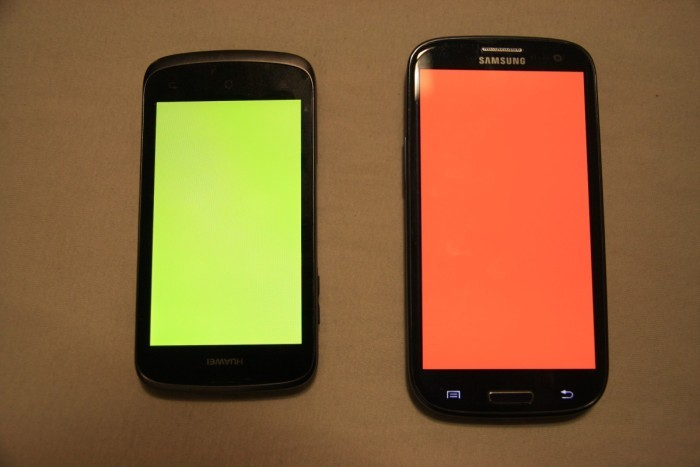
\includegraphics[width=\textwidth]{evaluation/IMG_7029.JPG}
                \caption{Colors of screens in light environment}
                \label{fig:tiger}
        \end{subfigure}
        ~ %add desired spacing between images, e. g. ~, \quad, \qquad etc.
          %(or a blank line to force the subfigure onto a new line)
        \begin{subfigure}[b]{0.4\textwidth}
                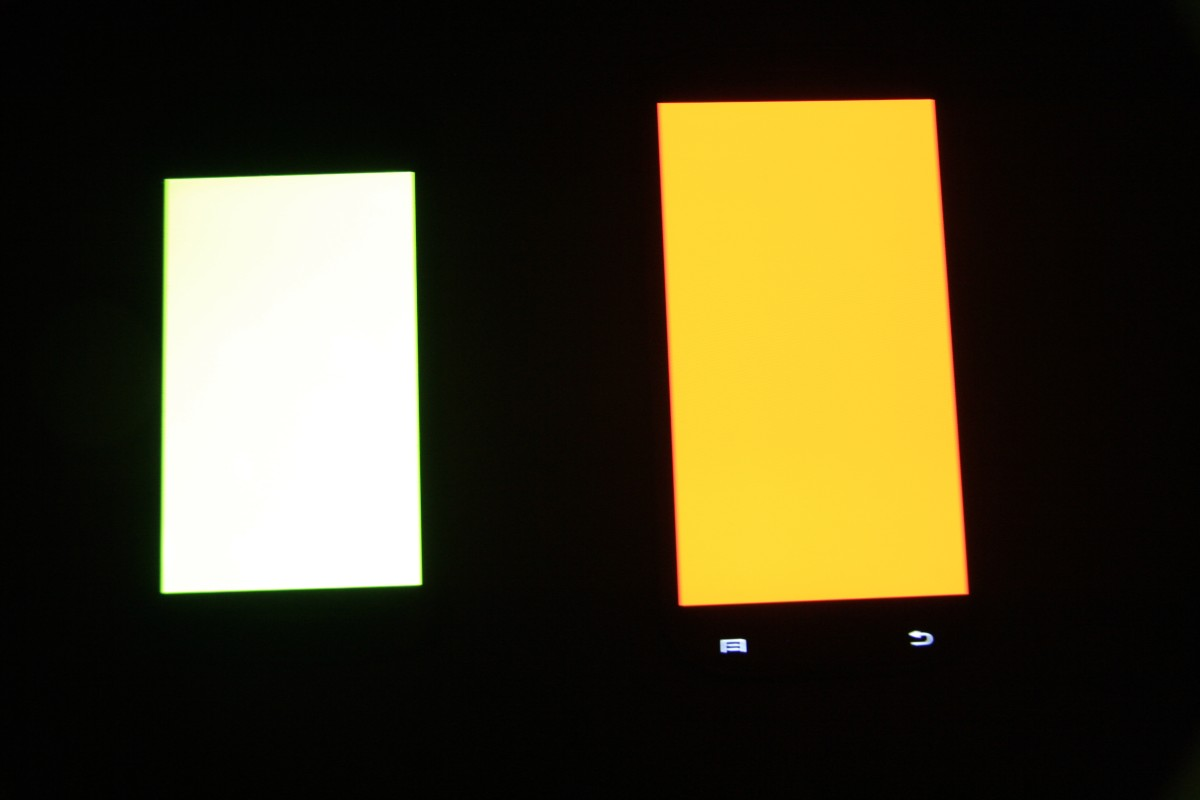
\includegraphics[width=\textwidth]{evaluation/IMG_7032.JPG}
                \caption{Colors of screens in dark environment}
                \label{fig:mouse}
        \end{subfigure}
        \caption{Colors of screens in different light environments}\label{fig:screen_colors_in_enviroments}
\end{figure}
By empirical research there were established colors (e. g. blue and white) which are least affected by this behavior.
